\chapter{Implementazione}
\label{cap:nomePrimoCapitoloTesi}
\lhead{\textbf{\rightmark}}

\indent{
	In questo capitolo è descritta l'implementazione del modello affrontato nelle metodologie.
	\newline
	Il nome scelto per l'applicazione finale realizzata è Naevus.\footnote{Vedi Appendice A per informazioni sul nome}
	\newline
	Naevus è stata svilupatta secondo un paradigma client/server.
	L'applicazione client è stata sviluppata con il framework Ionic/angular, mentre l'applicazione server con Django/python.
	\newpage
	\section{Architettura dell'applicazione Client-Server}
Il sistema è stato costruito secondo un'architettura Two-tyer, Client-Server.
\begin{figure}[h]
	\begin{center}
		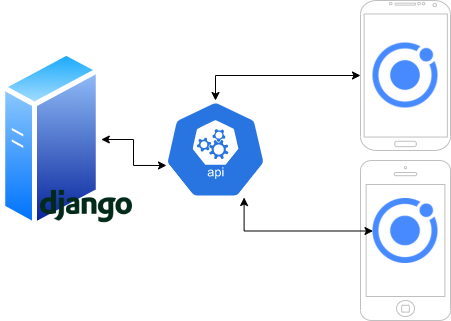
\includegraphics[scale=0.75]{figure/capitolo4/architettura1.png}
	\end{center}
	\caption{Illustrazione semplificata architettura del sistema proposto.}	
\end{figure}
\newline
L'applicazione client, sul device, presenterà all'utente i servizi di cattura dell'immagine ed i risultati dell'elaborazione avvenuta sul server con le informazioni annesse inviate tramite un metodo di comunicazione asincrono request–response; la comunicazione tra device e server avviene grazie ad un API di comunicazione presente sul device.
\begin{figure}[h]
	\begin{center}
		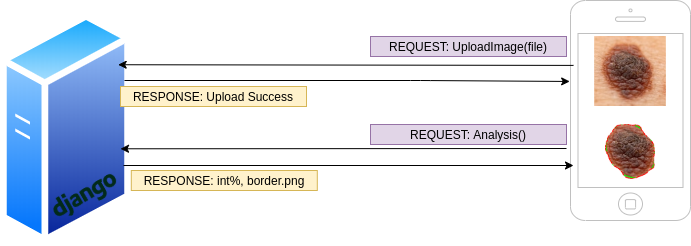
\includegraphics[scale=0.5]{figure/capitolo4/esempioarch.png}
	\end{center}
	\caption{Esempio semplificato di comunicazione Client-Server.}
\end{figure}
Per il layer di interfaccia presente sul device mobile è stato scelto il framework Ionic Angular al fine di creare un applicazione nativa cross-platform e quindi disponibile per device ios e android.
\newpage
L'architettura scelta sia per il client che per il server è stata progettata con un approccio modulare.
In questo modo l'inserimento di nuove applicazioni all'interno di django e conseguenzialmente all'interno dell'applicazione ionic è semplice e veloce, e non richiede necessariamente la conoscenza degli altri moduli che sono visti come unità blackbox.
La struttura interna di un modulo dipende in modo minimo dal “mondo esterno” e allo stesso tempo è possibile riutilizzare i moduli e svilupparli separatamente senza influenzare la struttura del codice degli altri moduli.
In questo modo se dovesse esserci un problema ad un singolo modulo gli altri non saranno influenzati (ad eccezione dell'applicazione che si occupa dell'upload dell'immagine che fornisce l'input dal quale parte l'intera analisi).
All'interno dei moduli è garantito un alto grado di modificabilità, estendibilità e di conseguenza, anche quanto detto in precedenza, è possibile aggiungere un numero indefinito di prototipi testabili anche separatamente.
\newline
Un design siffatto garantisce una low coupling – high cohesion, poiché le interazioni tra moduli sono limitate al minimo, garantendo riuso e modificabilità e di conseguenza anche manutenibilità del codice.
\newpage
\section{Sistema Proposto}
Il sistema dovrà offrire all'utente la possibilità di analizzare il nevo attraverso la camera dello smartphone ed in particolare offrire un'interfaccia di facile utilizzo e semplificata in modo da rendere gradevole e non complesso l'utilizzo dell'applicazione.
\subsection{Requisiti Funzionali}
I requisiti funzionali sono stati prodotti analizzando i lavori già esistenti e le metodologie descritte nel capitolo precedente.
\begin{itemize}
	\item \verb|RF_1| - Attiva Motore AR: Il sistema permette all'utente di attivare il motore AR per l'analisi del nevo con un click.
	\item \verb|RF_2| - Visualizza informazioni Nevo: Puntando sul nevo, il sistema inizia l'analisi del nevo.
	\item \verb|RF_3| - Visualizza Informazioni Nevo: Il sistema mostra all'utente le informazioni derivanti dall'anlisi del nevo. Le informazioni mostrate sono: asimmetria, bordo, colore, dimensione frattale, classificazione del nevo, diametro e distanza del centroide.
	\item \verb|RF_4| - Visualizza Aiuto: Il sistema permette all'utente di visualizzare la guida all'applicazione.
\end{itemize}
\newpage
\section{Design dell'applicazione client}
\subsection{AppModule}
Le applicazioni Angular possono utilizzare Cordova o Capacitor per creare app mobile native.
\newline
Nel caso specifico è stato scelto Cordova.
\newline
Per far questo è necessario importare il plug-in in @NgModule e aggiungerlo all'elenco dei provider.
\newline
Per Angular, il percorso di importazione dovrebbe terminare con /ngx. 
Il rilevamento delle modifiche di Angular viene gestito automaticamente.
Nell'applicazione Nevus progettata, sono stati utilizzati diversi plug-in al fine di fornire più funzionalità possibile lato applicazione.
I plug-in utilizzati, non standard, utilizzati nella progettazione sono:
\begin{itemize}
	\item CameraPreview da \textit{'@ionic-native/camera-preview/ngx'}:  rende disponibili le funzionalità della fotocamera per device android e ios.
	\item HttpClientModule da \textit{'@angular/common/http'}: permette l'utilizzo delle API di connessione con Django.
	\item ApiDjangoService da \textit{'./api-django.service'}: servizio creato ad hoc per la connessione con il server predisposto per l'analisi.
	\item NativeStorage da \textit{'@ionic-native/native-storage/ngx'}: permette l'utilizzo dello storage interno dell'applicazione.
	\item Base64ToGallery da \textit{'@ionic-native/base64-to-gallery/ngx';} permette il salvataggio dell'immagine scattata nella galleria del device.
	\item Crop da \textit{'@ionic-native/crop/ngx';} per il ritaglio dell'immagine scattata.
	\item PhotoViewer da \textit{'@ionic-native/photo-viewer/ngx';} permette la visione di un immagine a tutto schermo.
	\item File da \textit{'@ionic-native/file/ngx'} permette la creazione di file.
	\item Screenshot da \textit{'@ionic-native/screenshot/ngx'} permette di salvare schermate dell'applicazione.
\end{itemize}
\newpage
	\subsection {Design dell'Interfaccia}
Per lo sviluppo dell'interfaccia di "Naevus" sono state prese in esame applicazioni esistenti.
Tutte le applicazioni prese in esame hanno mostrato un numero notevole di interazioni tra applicazione e utente.
Per garantire la miglior usabilità possibile, Naevus è stata progettata in modo da garantire le  10 euristiche di Nielsen \cite{nielsen2005ten}, offrendo così un interfaccia semplice ed un estetica minimalista, garantendo corrispondenza tra mondo reale e mondo in realtà aumentata.
\newline
Il sistema è dotato di tre tipologie di interfaccia incluse in un unica interfaccia principale:
\newline
un'interfaccia pre-analisi in cui parte il motore di riconoscimento, un'interfaccia di informazione sull'utilizzo e un interfaccia di analisi che mostra le informazioni in continuo aggiornamento in realtà aumentata.
\subsection{Interfaccia pre-analisi}
Per la creazione dell'interfaccia dell'applicazione è stata utilizzata una struttura a griglia in un'unica schermata, con 2 pulsanti, in modo da rendere semplice l'utilizzo dell'applicazione anche a persone poco pratiche con la tecnologia.
\newpage
\begin{figure}[h]
	\begin{center}
		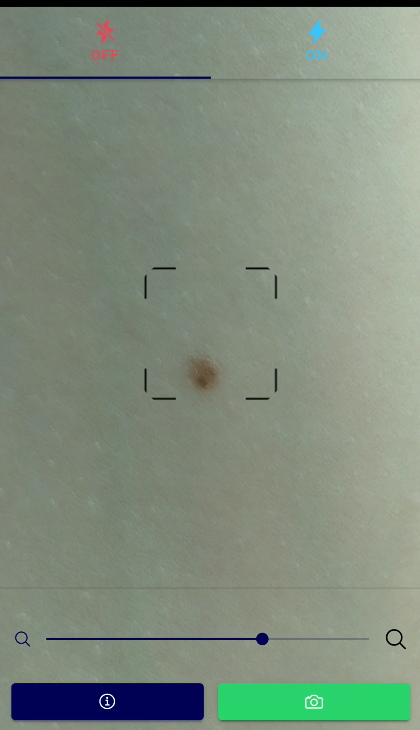
\includegraphics[scale=0.7]{figure/capitolo4/interface.png}
	\end{center}
	\caption{Schermata applicazione pre-analisi}
\end{figure}

Dall'interfaccia, visibile nella figura precedente, è possibile accendere o spegnere il flash del device ed effettuare uno zoom digitale fino a x25 \footnote{Lo zoom digitale di x25 garantisce un compromesso ideale tra zoom e qualità dell'immagine, l'aumento dello zoom troppo elevato può portare ad una perdita di qualità dell'immagine ed una difficoltà maggiore nella segmentazione del nevo da parte del server.}
\newline
Il flash è stato posizionato nell'header (in alto) dell'applicazione, in questo modo è lontano dalla zona focale situata al centro dello schermo. 
Lo zoom e il pulsante dello scatto sono stati situati in basso, in questo modo, l'utilizzo dell'applicazione può avvenire anche con una sola mano, il dermatologo o chi utilizza l'applicazione può utilizzare la mano sinistra per stabilizzare il punto ove si trova il nevo e la mano destra per scattare la foto; la medesima operazione può essere fatta anche da una persona mancina.
\newline
Prima dell'analisi è necessario far rientrare il nevo da analizzare nel mirino centrale. In questo modo l'applicazione effettuerà il ritaglio (crop) dell'immagine all'interno del mirino al fine di semplificare il lavoro del server di pulizia dei peli e segmentazione che sono onerosi.
\newpage
\subsection{Interfaccia Informazioni}
L'interfaccia informazioni offre all'utente una guida semplice ed intuitiva per l'utilizzo dell'applicazione.
\begin{figure}[h]
	\begin{center}
		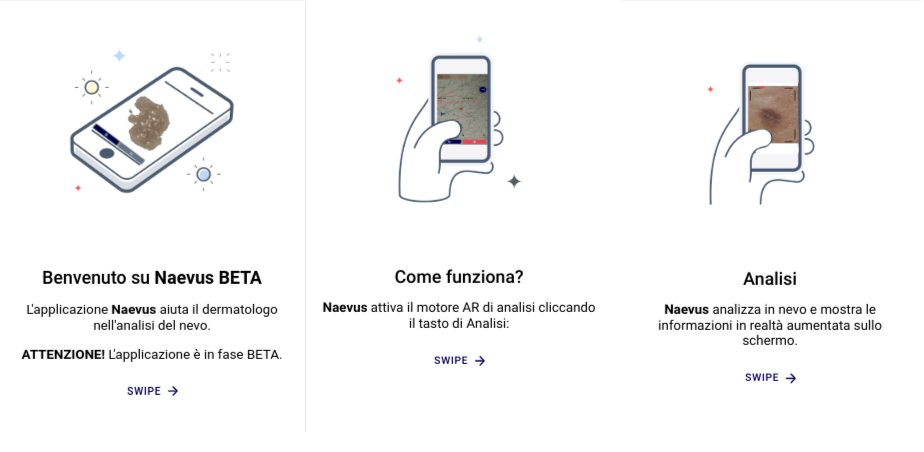
\includegraphics[scale=0.32]{figure/capitolo5/loading.png}
	\end{center}
	\caption{Schermate guida  all'applicazione}	
\end{figure}

\newpage
\subsection{Interfaccia Analisi}
L'interfaccia di Analisi in Realtà Aumentata offre all'utente la possibilità di osservare il nevo con la camera e di visualizzare le informazioni elaborate sul nevo intorno ad esso.
\begin{figure}[h]
	\begin{center}
			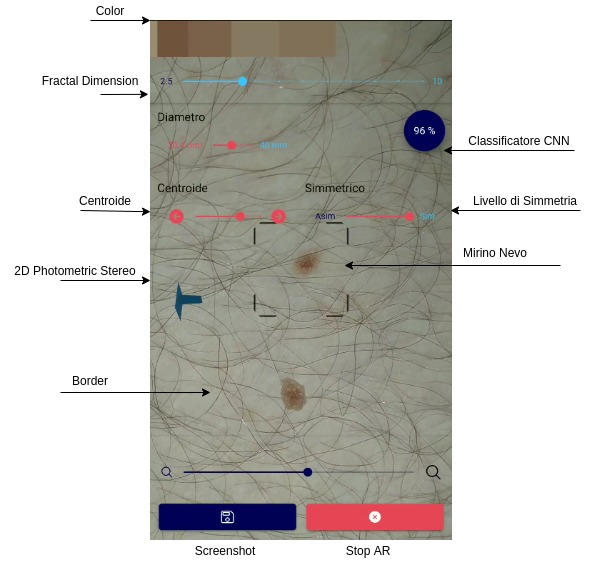
\includegraphics[scale=0.7]{figure/capitolo5/ui.jpg}
	\end{center}
	\caption{Schermate di caricamento dell'applicazione}	
\end{figure}
\newpage
Come mostrato nella figura precendente, all'interno dell'interfaccia di analisi sono presenti le caratteristiche ABCD.
All'interno dell'interfaccia è visibile, la lista dei colori assunti dal nevo sotto forma di immagine, la dimensione frattale, la dimensione del centroide, il livello di asimmetria/simmetria, la visione in 2D del nevo in modo da simulare la palpazione da parte del dermatologo, il bordo del nevo, il risultato prodotto dal classificatore H5 e la possibilità di effettuare zoom sul nevo.
Inoltre sono presenti due bottoni sul fondo, per salvare lo screenshot dell'analisi e per disattivare il motore AR.
\subsection{Photo Viewer}
Per dare la possibilità al dermatologo di visionare in dettaglio il bordo del nevo e la 2D photometric stereo, è stato implementato il plugin Photo Viewer che consente la visione a schermo pieno dell'immagine, come da esempio nella figura seguente.
Cliccando sul bordo del nevo, o sull'immagine 2D photometric stereo è possibile visionarle in alta definizione a schermo intero.
\begin{figure}[h]
	\begin{center}
		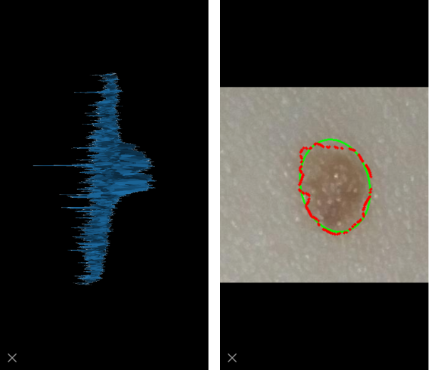
\includegraphics[scale=0.7]{figure/capitolo5/photoviewer.png}
	\end{center}
	\caption{Immagine 2D Photometric Stereo e Nevo con bordi evidenziati ed ellisse disegnata.}	
\end{figure}
\newpage
\subsection{Logica dell'interfaccia}
Per quanto concerne la logica dell'interfaccia, all'interno dei file typescript sono presenti gran parte dei comandi che consentono un utilizzo dinamico dell'interfaccia.
Le variabili sono definite prima del costruttore come da prassi fare in typescript.
\subsubsection{Camera Preview}
\textbf{CameraPreview} consente di utilizzare la fotocamera, anteriore e posteriore del device.
Viene impostato un valore base dello zoom \textit{setZoom} = 1;
Per quanto concerne la messa a fuoco dell'immagine, aspetto fondamentale di questa applicazione è stato preferito impostare una messa a fuoco semi-automatica da parte dell'utente che al click sullo schermo mette a fuoco il punto in cui si tocca oppure è la camera stessa a mettere a fuoco un oggetto che si trova al centro del mirino, in questo modo è l'utente stesso a capire se il livello di focus soddisfa o meno la visibilità del nevo;
\newline
la variabile che è stata utilizzata a tal scopo è \textit{tapfocus = false} con una impostazione semi automatica della messa a fuoco impostata tramite la variabile \textit{focusMode = 'auto';}
\newline
La Fotocamera viene attivata dal metodo \textit{async startCameraAbove()} che prova l'attivazione della camera definendo le impostazioni standard e impostando la camera posteriore (rear).
\newline
Lo scatto viene effettuato secondo impostazioni standard della fotocamera, con una risoluzione di 1280x1280 con una qualità del 100\%, senza compressione. 
\newline
L'immagine viene prima convertita in base64 e resa visibile come immagine e poi trasforamta da string base 64 a blob.
\newline
Infine il metodo \textit{base64ToGallery} permette all'app di salvare la foto appena scattata sul device.
\newline
\subsubsection{Refresh delle immagini}
Uno dei più noti problemi di ionic/angular è la difficoltà nel refresh dell'immagine quando il link di un immagine è lo stesso e l'immagine cambia, spesso ionic salva per un certo tempo le immagini di un link in cache, quindi anche quando si ricarica l'immagine; quindi anche se il refresh è attivo l'immagine viene presa dalla cache, per risolvere questo problema è stato utilizzato un trucco, ovvero un numero casuale preceduto da \textit{?} in modo da garantire il refresh anche quando si avvia una nuova analisi.
\begin{lstlisting}
...(path + "?" + (Math.random() * 3));
\end{lstlisting}
\newpage
\subsection{Servizi}
I servizi in Ionic/Angular sono dei file typescript che semplificato operazioni ricorrenti all'interno del progetto, in questo caso fungono anche da API di comunicazione con il server Django.
\subsubsection{uploading.service}
La logica di connessione per l'invio del file dal client al server è contenuta nel servizio \textbf{uploading.service.ts}.
Il servizio utilizza il plugin \textit{HttpClient} di \textit{'@angular/common/http'} e permette la comunicazione tramite richieste request-response.
\begin{lstlisting}
DJANGO_API_SERVER: string = "http://192.168.1.13:8000";
constructor(private http: HttpClient) { }

public uploadFormData(formData) {
return this.http.post<any>(`${this.DJANGO_API_SERVER}/upload/`, formData);
}
\end{lstlisting}
Quindi tramite il metodo \textit{uploadFormData} con una chiamata post viene inviata la form contenente il file da caricare. E ritorna il messaggio di successo o insuccesso dell'upload.
\subsubsection{apidjango.service}
La logica di connessione per l'invio di richieste dal client al server è contenuta nel servizio \textbf{apidjango.service.ts}.
Qui sono contenuti tutti i metodi per le chiamate alle singole applicazioni di django che si occuperanno delle analisi ed estrazioni delle caratteristiche del nevo.
In particolare:
\begin{itemize}
	\item getClassified: si occupa di lanciare la rete neurale che effettuerà l'analisi sul nevo per il riconoscimento di un melanoma.
	\item getAsymmetry: si occuapa di lanciare l'analisi per l'asimmetria del nevo e la 2D photometric stereo e torna in output un valore float.
	\item getBorder: si occupa del preprocessing e torna in output il valore del classificatore della rete neurale.
	\item getColor: si occupa dell'analisi per colore del nevo e torna in output la dimensione frattale e l'immagine dei colori.
	\item getCentroid: si occupa dell'analisi del centroid e ritorna un valore float.
	\item clearPic: si occupa della pulizia dopo l'analisi di un nevo. 
\end{itemize}
\newpage
\section{Design dell'applicazione server}
Django è un framework Web Python di alto livello che incoraggia lo sviluppo rapido e un design pulito e pragmatico ed è uno strumento gratuito e open source.
\newline
Django è stato progettato per rendere semplici e veloci le attività di sviluppo Web comuni.
Un progetto Django ha la seguente architettura,
Django ha un design standard il cui punto di forza è la possibilità di aggiungere un numero indefinito di applicazioni ed eseguirle singolarmente, in questo modo si può sfruttare al meglio il parallelismo e la possibilità di ricevere i risultati delle feature singolarmente, riducendo i tempi di analisi.
\newpage
\subsection{Struttura dell'applicazione}
L'albero dell'applicazione è strutturato nel seguente modo:
\begin{lstlisting}
backendNevus/
	manage.py
	core/
		__init__.py
		settings.py
		urls.py
		wsgi.py
		uploadapp/
	__init__.py
	admin.py
	apps.py
	models.py
	serializers.py
	tests.py
	urls.py
	views.py
border/
	[...]
	views.py
asymmetry/
	[...]
	views.py
centroid/
	[...]
	views.py
classifier/
	[...]
	views.py
color/
	[...]
	views.py
clearpic/
	[...]
	views.py
media/
\end{lstlisting}

\subsubsection{core}
Nel core dell'applicazione sono presenti gli url delle applicazioni e il collegamento alla cartella Media dove saranno salvati i file di upload ed elaborazione.
\subsection{uploadapp}
L'applicazione \textbf{uploadapp} consente l'upload da parte del dispositivo mobile, in particolare l'interfaccia visibile dall'applicazione è offerta al file \textit{views.py}:
\newpage
\subsection{Analisi del Nevo}
Nelle sezioni successive è possibile vedere come i modelli definiti nelle metodologie sono stati implementati nell'applicazione Server finale.
\newline
\subsection{border}
L'applicazione \textbf{border} si occupa del preprocessing dell'immagine caricata sul server e del ritaglio di quest'ultima, mettendo in evidenza i bordi e costruendoci sopra un ellisse che raccolga i bordi e simuli un cerchio sul nevo.
Si occupa inoltre dell'utilizzo del classificatore h5.
\subsubsection{Rimozione Peli}
Il preprocessing si occupa della pulizia dei peli dell'immagine.
Il primo procedimento è la conversione dell'immagine in grayscale, poi costruisce il kernel con un filtro morfologico, e infine vengono intensificati i peli.
\begin{figure}[h]
	\begin{center}
		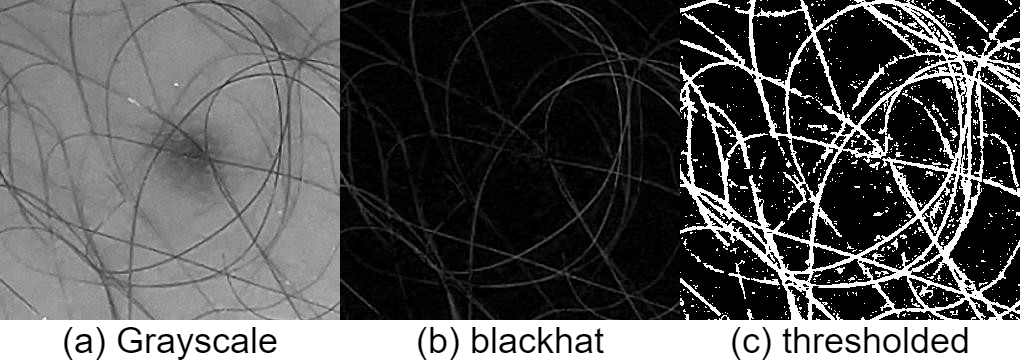
\includegraphics[scale=0.4]{figure/capitolo6/border1.png}
	\end{center}
	\caption{Preprocessing rimozione peli}	
\end{figure}
\begin{figure}[h]
	\begin{center}
		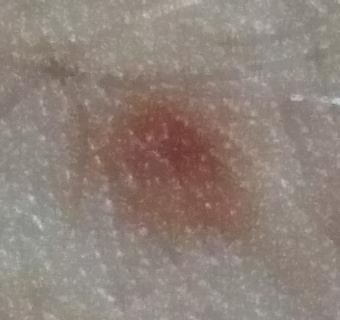
\includegraphics[scale=0.4]{figure/capitolo6/border2.jpg}
	\end{center}
	\caption{Immagine finale rimozione peli}	
\end{figure}
La scelta di inserire un valore elevato per la pulizia dei peli è dovuto alla difficoltà nei test iniziali di pulire i peli quando questi sono molto spessi e scuri. Questo scelta non influenza l'immagine priva di peli o con peli sottili ma può portare a una perdita di qualità dell'immagine quando molti peli sono sovrapposti al nevo, per cui la scelta di intensificare la rimozione dei peli ha portato una maggiore qualità quando i peli sono molto scuri come in figura 6.7; ad ogni modo si può notare che nell'immagine finale ci sono comunque tracce minime di peli come visibile in figura 6.8.
\newpage
\subsubsection{Segmentazione}
Come per la rimozione dei peli, anche per la segmentazione ho seguito un procedimento diverso rispetto a quello descritto nel Capitolo 3 di questa tesi, essendo le immagini non prodotte da un dermatoscopio digitale ma dalla camera di uno smartphone.
\newline
Le figure 6.9 da (a) a (c) mostrano le prime fasi di costruzione dell'immagine in cui viene applicato prima un filtro \textit{bgr2hsv}, in secondo luogo un filtro \textit{bgr2gray}, ed infine il \textit{blur} dell'immagine.
\newline
Infine vengono selezionati i contorni del nevo dall'immagine, e viene effettuato il ritaglio del nevo, ed in parallelo vengono evidenziati i bordi (colore rosso) e viene costruita un'ellisse a ricoprire la circonferenza del nevo (figura 6.9 (d)). 
\begin{figure}[h]
	\begin{center}
		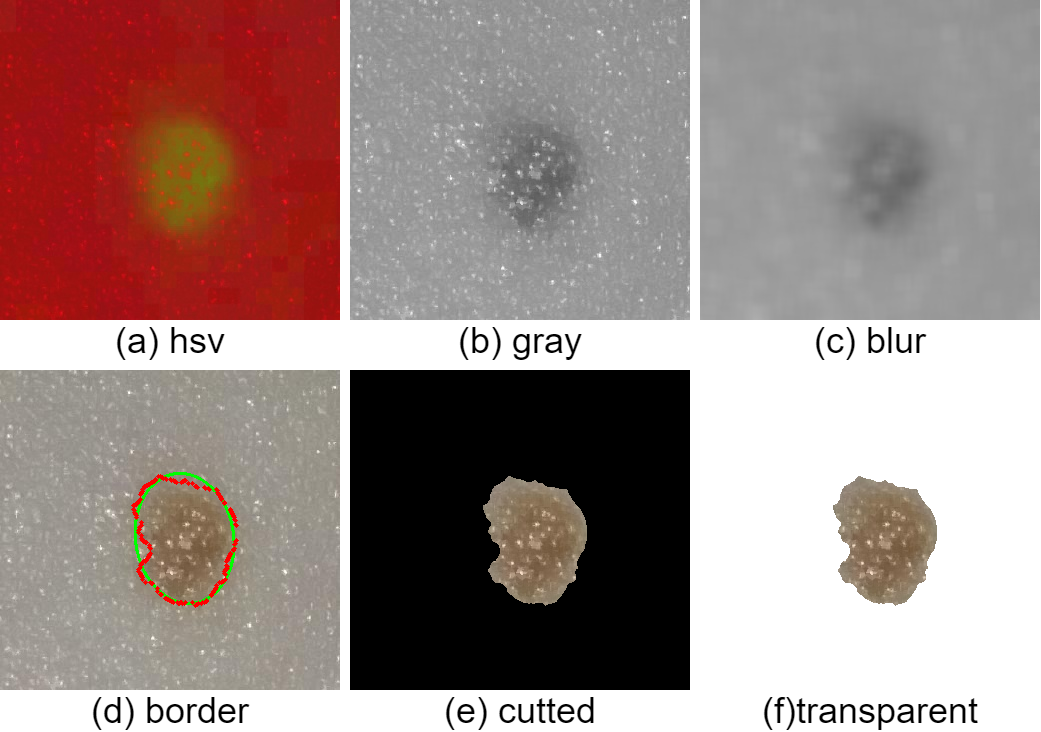
\includegraphics[scale=0.3]{figure/capitolo6/borderlist.png}
	\end{center}
	\caption{Immagine finale rimozione peli}	
\end{figure}
\newpage
\subsubsection{black remove}
L'ultima operazione richiede la rimozione del nero prodotto dalla segmentazione, per fare questo si utilizza un semplice algoritmo che trova i pixel neri e li trasforma in trasparenti; quindi il bordo viene trasformato per rendere il contorno dell'immagine trasparente (figura 6.9(e)). La trasformazione è stata fatta con il seguente algoritmo:
\begin{lstlisting}
for item in datas:
if item[0] < 3 and item[1] < 3 and item[2] < 3:
newData.append((255, 255, 255, 0))
else:
newData.append(item)
\end{lstlisting}
\begin{figure}[h]
	\begin{center}
		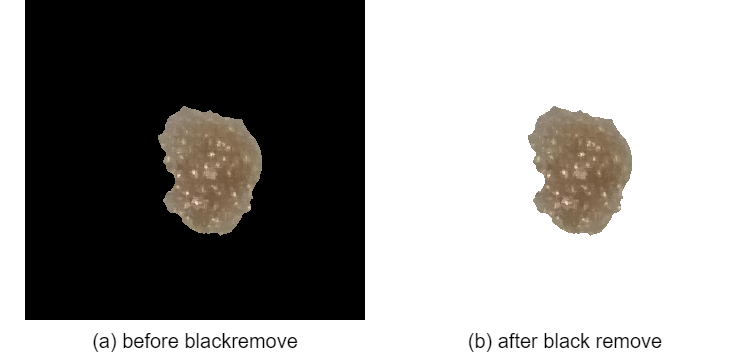
\includegraphics[scale=0.5]{figure/capitolo6/blackremove.png}
	\end{center}
	\caption{Prima e dopo l'esecuzione dell'algoritmo \textbf{black remove}}	
\end{figure}
\newpage
\subsection{asymmetry}
L'applicazione \textbf{asymmetry} calcola il livello di asimmetria del nevo e genera l'immagine 3D del nevo.
\subsubsection{asimmetria}
L'algoritmo utilizzato per calcolare l'\textbf{asimmetria} è basato sull'immagine prodotta dall'applicazione \textbf{border}.
Tramite l'ellisse che viene costruita nell'immagine in figura 6.9 (d), viene calcolata l'asimmetria del nevo. In questo modo è semplice verificare anche visivamente da parte da parte del dermatologo il livello di asimmetria.
\newline
\subsubsection{2D photometric stereo}
L'algoritmo per la trasformazione in 2D photomeric stereo prende in input l'immagine in figura 6.9(e) e la trasforma in 3D su un piano 2D.
\newpage
\subsection{classification}
Questa applicazione si occupa di calcolare la percentuale di probabilità che il nevo sia un melanoma o meno utilizzando la rete neurale convoluzionale descritta nel capitolo 3 di questa tesi.
L'immagine viene prima processata sulla dimensione per essere compatibile con il classificatore e poi data in input a quest'ultimo.
L'immagine che viene presa in input prima dell'elaborazione è quella prodotta dall'applicazione \textbf{border} figura 6.9 (e).
Il risultato dell'elaborazione (valore float da 0 a 1) viene convertito in intero ed in percentuale.
\newpage
\subsection{centroid}
L'applicazione \textbf{centroid} produce il centroide del nevo.
In valore è espresso in un range compreso tra 0 e 1 in cui 0.5 rappresenta la distanza del centroide calcolata mediante le coordinate x e y del centroide al fine di ottenere un valore compreso tra 0 e 10, se il centroide è uguale a 5 corrisponde al centro del nevo all'interno dell'ellisse.
\subsection{color}
L'applicazione \textbf{color} analizza i colori dell'immagine datagli in input e produce la percentuale di colore per ogni colore, e l'immagine con i colori più presenti all'interno dell'immagine, il numero di colori da cercare sotto forma di cluster scelto è pari a 5, questo perché un numero troppo elevato di cluster rallenta molto l'esecuzione dell'applicazione \textbf{color}.
L'immagine che prende in input color è border (figura 6.9 (e))
Il codice prevede un primo algoritmo in cui vengono indicati il numero di cluster e la chiamata a funzione che si occupa di selezionare solo i colori che hanno una percentuale minore del 70\%, questo perché altrimenti verrebbe selezionato anche il nero che fa da sfondo all'immagine.
\newline
La funzione visualize\_colors prende in input cluster e cluster.centers ed in output produce il rettangolo costruito con i cluster (di colori) che hanno percentuale inferiore al 70\% e la percentuale di colore per ogni cluster.
Se la percentuale di nero dovesse essere minore al 70\% l'immagine viene pulita da un algoritmo che analizza i singoli pixel alla ricerca del colore nero [0, 0, 0] e li rimuove dall'immagine.
L'immagine finale prodotta è presente nella figura 6.11
\begin{figure}[h]
	\begin{center}
		
\includegraphics[scale=0.5]{figure/capitolo6/color.png}
	\end{center}
	\caption{Scala di colori prodotta dall'applicazione \textbf{color}}	
\end{figure}
\newpage
\subsection{clearpic}
Clearpic è un'applicazione che mira a pulire il server dalle immagini presenti in cache, in modo da garantire un continuo e corretto funzionamento del server, dopo o prima di una analisi.
L'applicazione viene eseguita sia dal server stesso che lanciata dall'applicazione client.
Inoltre verifica la presenza dei file prodotti dall'analisi nella cartella \textit{/media} e li elimina, garantendo la possibilità di effettuare una nuova analisi.
\newpage
\subsection{diameter}
L'applicazione \textbf{diameter} prende in input l'immagine border figura 6.9 (f) e lo zoom del device e calcola il diametro del nevo.
Il calcolo del diametro richiede la trasformazione dell'immagine in gray e poi viene effettuato il blur.
Vengono costruite 4 linee intorno al nevo che costituiranno un rettangolo, dopodiché vengono costruiti 6 marker intorno al rettangolo appena costruito che saranno utilizzati per calcolare i due diametri ovvero base ed altezza del rettangolo.
Il risultato finale viene prima convertito da pollici in millimetri \footnote{1 Pollice corrisponde a 25,4 millimetri.}, ed in un secondo momento diviso per una costante pari a 100 al fine di rendere i dati significativi, infine per calcolare il diametro finale viene fatto il rapporto tra la base e l'altezza del rettangolo diviso 2.
Il risultato ottenuto è un'approssimazione del diametro, con un buon margine di errore. Nella figura sottostante è possibile notare il procedimento di analisi del nevo al fine di calcolare il diametro.
\begin{figure}[h]
	\begin{center}
		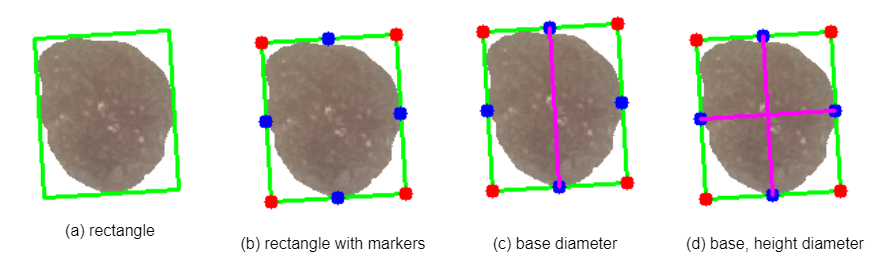
\includegraphics[scale=0.47]{figure/capitolo6/diameter.png}
			\end{center}
	\caption{Passi per il calcolo del \textbf{diametro}}	
\end{figure}

}